\chapter{On the Hales-Jewett theorem}

In this chapter, some notions about the Hales-Jewett theorem are presented. Firstly, we start with some basic notions on arithmetic progression, which are important for understanding the next point. After, we introduce some elementary notions about the Van der Waerden’s theorem and the Szemerédi's theorem. We highlight that  the Van der Waerden's theorem is a particular case of the  Szemerédi's theorem. Ultimately, we present the two forms of the Hales-Jewett theorem and link these one to the two first theorems.

\section{Arithmetic progression}


\begin{defn}
Let $a_1, a_2, \ldots, a_n$ be a sequence of numbers.  

This sequence of numbers forms an \textbf{arithmetic sequence} if every term of this sequence is obtained by adding a constant to the previous term.
\end{defn}
The constant is simply the difference between two consecutive terms.

If $a_1$ and $a_n$ represent the first and the $n$-th term of a sequence, and $d$ the constant, then the general term $a_n$ of this sequence is expressed as:

$$a_n=a_1+(n-1)d.$$

Knowing $a_m$ and the constant $d$, then $a_n$ can be expressed as:
 
$$a_n=a_m+(n-m)d.$$

\subsection{Arithmetic progression of length k}


Let $a$ and $d$ be two fixed numbers.

An arithmetic progression of length k is an arithmetic sequence of $k$ numbers of the form $a+nd.$ $a$ is the first term of the arithmetic progression, $d$ is the difference between two consecutive terms and $n=0,1, \ldots, k-1$, that is, we have $k$ consecutive values of $n.$ 

We denote by AP$(k)$ or AP$-k$ or $k-$AP, the arithmetic progression of length $k.$


\section{Van der Waerden's theorem}

Before stating the Van der Waerden's theorem, let us introduce and define some concepts and notation.

A \textit{partition} of a set $A$ is a collection of nonempty and mutually disjoint subsets $A_i$ of $A$, such that  $A=\cup A_i$ and $A_i \cap A_j=\emptyset, \quad i\neq j.$ Thus, a partition is also a sequence $A_1, A_2, \ldots, A_n$ of mutually nonempty and  disjoint subsets of set $A$. $A_i$ are known as \textit{blocks}.

We denote by $\mathbb{Z}^+$, the set of positive integers.
Let $m \in \mathbb{Z}^+$, we designate by $[m]$ the set $\{1,2, \ldots, m\}.$
%\Jnote{Use ldots instead of cdots}.

Let $X$ be a set and $r$ be a positive integer. We want to colour elements of set $X$ with $r$ colours. If $C$ represents the set of colours, then $|C|=r$ is the number of colours.

\begin{defn} An $r$-colouring of $X$ is a mapping $c \ : \ X \longrightarrow [r].$  \label{rcol}\end{defn}
%\Jnote{Still a problem here: You should write \$r\$-coloring, with - outside math mode.}


If $|X|=n$, then the number of $r$-colorings of $X$ is $n^r.$

%\Jnote{Better: ``the number of $r$-colorings of $X$ is''}

Let $Y$ be a subset of $X.$ We say that $Y$ is \textit{monochromatic} when the restriction $c\restriction_Y$ is constant, that is   if $c(y)$ is the same for every $y \in Y.$

%\Jnote{For restriction better use \textbackslash restriction and write $Y$
  %in lower script, like this: $c\restriction_Y$.}

According to \cite{polymath2012new}, the Van der Waerden's theorem is stated as follows:

\begin{thm}[Van der Waerden]
For every pair $(k,r) \in \mathbb{Z}^+ \times \mathbb{Z}^+$, there exists $N_0 \in \mathbb{Z}^+$ such that for every $N \geq N_0$ and for 
every $r$-colouring of $[N]$ there is a monochromatic arithmetic progression of length $k.$  \label{vd1}
\end{thm}

%\Jnote{I think it is more consistent with other theorems to state this as:
  %``there exists $N_0$ such that for every $N \ge N_0$''}

We know that an $r$-colouring is a function called $c$ in definition \eqref{rcol}. So, in other words we can find at least one subset of $\{1,2,\ldots,N\}$ with $k-$elements such that all elements have the same colour and form an arithmetic progression of length $k$. That is, there exist
%\Jnote{s/exit/exist}
$a$,  $d \ \in \mathbb{N}$ with $d\neq 0$ such that: $c(a)=c(a+d)=c(a+2d)=\ldots =c(a+(k-1)d)$ where $a, a+2d, \ldots, a+(k-1)d$ are elements of the subset.

The Van der Waerden's theorem can also be formulated using partition \citep{dransfield2004} as:

\begin{thm}[Van der Waerden]
For every $k, r \in \mathbb{Z}^+$ , there exists $N_0 \in \mathbb{Z}^+$ such that for every $N \geq N_0$ and for every partition $A_1, \ldots , A_r$ of $[N]$, there is $i$, $1 \leq i \leq r$, such that the block $A_i$ contains an arithmetic progression of  length $k.$   \label{vd2}
\end{thm}

Note that for this version a block in a partition can be empty. Thus, in many cases in this essay a block can be empty.

The existence of the number $N_0$ for which any $r$-colouring of the integer $\{1, \ldots, N_0 \}$ is certain to have a monochromatic subset of cardinality $k$ of which elements form an arithmetic progression was demonstrated constructively in 1927 by Bartel Leendert Van der Waerden  \citep{van1927beweis}. 
\cite{graham1974short} gave \emph{another} proof of this theorem. The book entitled "\textit{Purely Combinatorial Proofs of Van der Waerden-Type Theorem}" written by \cite{gasarch2010purely} condenses  the proof of Van der Waerden theorem.
%\Jnote{Be careful with capitalization: it is   ``Van der Waerden's theorem''.}

In this theorem, to find the number $N$ even showing that $N$ is not trivial are difficult. The least such number $N_0$ is called \textit{Van der Waerden number} denoted as $W(k,r).$ In the rest of this chapter, we will use $W(k,r)$ or simply $W$ to denote the least Van der Waerden number instead of $N_0.$

The general expression of $W(k,r)$ is not known, but for some $k$ and $r$ there are exact values known or there are some approximations of the  lower or upper bound of $W(k,r)$  \citep{dransfield2004}.

$W(1,r), \ W(k,1)$ and $W(2,r)$ are known as \textit{trivial} Van der Waerden numbers. So, 
\begin{itemize}
\item $W(1,r)=1$:  the set of all subsets of a nonempty set contains necessary a singleton. A singleton forms an arithmetic progression of length $1$ where the difference between two consecutive numbers is $0.$ To form a monochromatic arithmetic progression of length $1$ by $r$-colouring a set, we need  a set of at least one element. 
\item $W(k,1)=k$: by colouring a set with one colour, we automatically get a monochromatic arithmetic progression of length equals to the cardinality  of the set.
\item $W(2,r)=r+1$: to obtain a monochromatic arithmetic progression of length $2$ by $r$-colouring a set, we need a set of at least $r+1$ elements.
\end{itemize}

For instance, let us find the Van der Waerden number $W(3,2)$, that is an number $W(3,2)$ such that every $2$-colouring  of the set $[W(3,2)]$ contains a monochromatic arithmetic progression of length $3.$
%\Jnote{Rephrase: ...that is $N_0$ such that every $2$-coloring of $[N_0]$   contains a monochromatic...}

The value of $W(3,2)$ is greater than $8$ because for any $2$-colouring of $[n],\ n\in \{3,4,5,6,7,8\}$, we can find a $2$-colouring which does not contain a monochromatic arithmetic progression of length 3. For instance, the set  $\{1,2,\ldots, 8\}$ does not contain a monochromatic  arithmetic progression of length $3$ by $2$-colouring the set  like in the table \eqref{van23}. The table \eqref{van23} has been adapted from  \cite{wiki:Van_der_Waerden's_theorem}.
So, when $W(3,2)=9$ we always find a monochromatic arithmetic progression of length 3 for any $2$-colouring of the set  $\{1,2,3,4,5,6,7,8,9\}.$ The table \eqref{van23} shows one of the possibilities of colouring of the  $\{1,2,3,4,5,6,7,8,9\}.$  If the ninth number is {\color{blue} blue}, then{ \color{blue}3, 6, 9}  form an arithmetic progression. If the ninth number is {\color{red} red}, then {\color{red}1, 5, 9} form an arithmetic progression. Therefore, by adding a ninth number and colouring it using any of the two colors, we always create  a monochromatic arithmetic progression of length 3.

\begin{table}[h]
\begin{center}
\begin{tabular}{ccccccccc}
\hline
1 & 2 & 3 & 4  & 5 & 6 & 7 & 8 & 9 \\ \hline
\color{red}R & \color{blue}B & \color{blue}B & \color{red}R & \color{red}R & \color{blue}B & \color{blue}B & \color{red}R  & \\
\hline 
\end{tabular} 
\end{center}
\caption{A $2-$colouring of $\{1,2,\ldots, 9\}$}
  \label{van23}
\end{table}

%\Jnote{This example is now very well explained!} 

The table \eqref{vdn} presents the 7 exact non-trivial Van der Waerden numbers  (when $k\geq 3$) \citep{dransfield2004}.

\begin{table}[h]

\begin{center}
\begin{tabular}{|c|c|c|c|}
\hline 
$k \setminus r$ & 2 & 3 & 4  \\ 
\hline 
3 & 9 & 27 & 76  \\ 
\hline 
4 & 35 & 293 &   \\ 
\hline 
5 & 178 &  &   \\ 
\hline 
6 & 1132 &  &   \\ 
\hline 

\end{tabular}
\end{center}
\caption{The 7 exact non-trivial values of Van der Waerden numbers.} \label{vdn}
\end{table} 

As related previously, searching for the exact value of $W(k,r)$ remains an open  problem.
%\Jnote{s/difficult/open and then delete next sentence.}
 The number $W(k,r)$ becomes hard to find when the values of $k$ and $r$ increase. However, for some $k$ and $r$ there is an approximation of the lower or upper bound of $W(k,r)$ \citep{stevens1978computer, herwig2007new, beeler1979some, dransfield2004, brown2008bounds, rabung2012, kouril2008van}. The table \eqref{vdw1} summarizes these known lower bounds and includes the seven non-trivial Van der Waerden numbers known exactly.

\begin{table}[h]
\begin{tabular}{|c||c|c|c|c|c|}
\hline 
$\mathbf{k \setminus r}$ & \textbf{ 2 }& \textbf{3} & \textbf{4} & \textbf{5} & \textbf{6} \\ 
\hline  \hline
\textbf{3}  &	9	& 27 &	76 &	 \textgreater  170 &	  \textgreater  223 \\ \hline 
\textbf{4}	& 35 &	293  &	 \textgreater 1,048 &	 \textgreater 2,254 &	 \textgreater  9,778 \\ \hline 
\textbf{5}	& 178	& \textgreater 2,173 &	 \textgreater 17,705 &	 \textgreater 98,740 &	 \textgreater 98,748 \\ \hline 
\textbf{6}	& 1,132 &	 \textgreater 11,191 & \textgreater 91,331 &	 \textgreater 540,025 &	 \textgreater  816,981 \\ \hline 
\textbf{7}	&  \textgreater 3,703 &	 \textgreater  48,811 &	 \textgreater 420,217 &	 \textgreater 1,381,687 &	 \textgreater 7,465,909 \\ \hline 
\textbf{8}	&  \textgreater 11,495 &	 \textgreater 238,400 &	 \textgreater 2,388,317&	 \textgreater 10,743,258&	 \textgreater 57,445,718\\ \hline 
\textbf{9}	&  \textgreater 41,265 &	 \textgreater 932,745&	 \textgreater 10,898,729&	 \textgreater 79,706,009&	 \textgreater 458,062,329 \\ \hline 
\textbf{10}	 &  \textgreater 103,474&	 \textgreater 4,173,724&	 \textgreater 76,049,218&	 \textgreater 542,694,970 &	 \textgreater 2,615,305,384 \\ \hline 
\textbf{11}	&  \textgreater 193,941&	 \textgreater 18,603,731&	 \textgreater 305,513,57 &	 \textgreater 2,967,283,511 &	 \textgreater 3,004,668,671 \\ \hline 
\end{tabular} 

\caption{Some lower bounds and exact non-trivial values of Van der Waerden numbers $W(k,r).$} \label{vdw1}
\end{table}

The estimation of lower and upper bounds is also an open problem. There exist some expressions that bound Van der Waerden numbers.  Researchers are still looking for closer bound or exact general expression of these numbers.
 \cite{erdos1952combinatorial}, cited by \cite{dransfield2004} established an inequality for the lower bound for $W(k,r).$
\begin{equation}
\left[2(k-1) r^{k-1} \right]^{\frac{1}{2}} < W(k,r). \label{erdos}
\end{equation}

\cite{brk1968} found a better bound when $k-1$ is a prime number  and for $r=2$. But these bounds still  require improvement. 
%\Jnote{Do not use symbols inside sentences,   write ``when $k-1$ is prime''.}
 \begin{equation}
 (k-1)2^{k-1}<W(k,2). \label{berlk}
 \end{equation}

Hence, for $p=k-1$, the expression \eqref{berlk} becomes:
 \begin{equation}
 p2^{p}<W(p+1,2). \label{berlk1}
\end{equation}
%\Jnote{Is $r$ above equal to two?}

So, $W(6,2) >5 \times 2^5=160$, $W(8,2) >7 \times 2^7= 896$ and $W(12,2) >11 \times 2^11= 22528.$
\citep{dransfield2004} improve this lower bound by using propositional satisfiability solvers  for some small Van der Waerden numbers, for instance $W( 8,2) > 1322$. \cite{rabung2012} performs more. Thus, as related in table \eqref{vdw1}, most of the lower bounds used, came from \cite{rabung2012}.

The best known upper bound of $W(k,r)$ is the expression  \eqref{gow} which came from the work of \cite{gowers2001new} on a  new proof of the Szemerédi's theorem. Section \eqref{sz} will talk about this theorem. The  Szemerédi's theorem is the extension of the Van der Waerden's theorem, that is the Van der Waerden's theorem is implied by the  Szemerédi's theorem.
%\Jnote{s/is a particular case/is implied by}
\begin{equation}
W(k,r) \leq 2^{2^{r^{2^{2^{k+9}}}}}     \label{gow}
\end{equation}

\section{Szemerédi's theorem} \label{sz}

The Szemerédi's theorem is merely another formulation of  the Van der Waerden's theorem in terms of \textit{density version}. Below, we show that the Szemerédi's theorem implies the Van der Waerden's theorem.

Let us consider $A$ a nonempty subset of the set $[N]$. The density of $A$ inside $[N]$ is a positive real number $\delta=\frac{|A|}{N}$. It is clear that $0< \delta \leq 1.$ 

The  theorem \eqref{sz1} is the famous Szemerédi’s theorem. Famous because the various proofs of the  Szemerédi's theorem connect disparate fields of mathematics (combinatorics, harmonic analysis, ergodic theory,  number theory, \ldots). \cite{arana2015depth} analysed the depth of the  Szemerédi's theorem by assembling the thoughts of some mathematicians (like Erdos and Terence Tao) about the major accomplishment of this theorem. According to \cite{polymath2012new}, the Szemerédi's theorem is formulated as:

\begin{thm}[Szemerédi's theorem]	For every  $k \in \mathbb{Z}^+$ and every $0< \delta \leq  1$ there exists an integer $N_0(k,\delta) \geq 1$ such that for every $N \geq N_0$ and every subset $A \subseteq [N]$ of size $|A|\geq \delta N$ contains an arithmetic progression of length $k.$  \label{sz1} \end{thm}
%\Jnote{Don't cite Polymath above. This is still not fixed. You can say something like ``according to polymath2012new''.}

The Szemerédi's theorem has a formulation which uses the notion of positive upper density. 

Let $A$ be a subset of the integers $\mathbb{Z}$ with positive upper  density, that is, satisfying 

$\lim \sup\limits_{N\rightarrow \infty} \frac{|A \cap[-N,N]|}{|[-N,N]|} > 0.$
%\Jnote{Put the formula on separate line.}
Then, for any $k \geq  1 $, $A$ contains infinitely many arithmetic progressions of length $k.$

As conjecture, the Szemerédi's theorem was formulated by \cite{JLMS}. There are several proofs of this theorem. The cases $k=1$ and $k=2$ are easy to prove. \cite{roth1953certain, roth1970irregularities} proved the case $k=3.$ The case $k=4$ was proved by \cite{szemeredi1969sets} and he gave the general case \citep{szemeredi1975sets}.

Some of proofs necessitated the use of other theories external to combinatorics. Thus, the ergodic theory (\textit{theory related to dynamical system with invariant measures and chaos theory})  has been used to prove this theorem by \cite*{furstenberg1977ergodic, furstenberg1982ergodic}.
%\Jnote{Use \textbackslash cite* to avoid et al.}
\cite{gowers1998fourier, gowers2001new}  used Fourier analysis and the inverse theory of additive  combinatorics to show this theorem. A few years later \cite{gowers2007hypergraph} used a hypergraph regularity lemma to prove this theorem. A  quantitative ergodic theory proof, version of \cite{furstenberg1982ergodic} has been presented  by \cite{tao2006quantitative} which does not involve some concepts used in the previous proofs: the axiom of choice, the use of infinite sets or measures, the use of the Fourier transform or inverse theorems from additive combinatorics.

\subsection{The Szemerédi's theorem implies the Van der Waerden's theorem.} \label{vsz}

\begin{proof}
  Let us assume that the Szemerédi's theorem \eqref{sz1} is true, that is $\forall k \in \mathbb{Z}^+$, $0< \delta \leq  1$, $\exists N_0(k,\delta) \in \mathbb{Z}^+/ \forall N \geq N_0$ and $ \forall A \subseteq [N]$, $|A|\geq \delta N$ contains an arithmetic progression of length $k.$ So, the aim is to show the  Van der Waerden's theorem from the Szemerédi's theorem. This means to  show that by $r$-colouring the set $\{1,2,\ldots, N\}$, we obtain at least one monochromatic arithmetic progression of length $k.$
  
   Let us notice that we have shown \eqref{vd1} and \eqref{vd2} that $r$-colouring a set  is to partition it to $r$ blocks.
 % \Jnote{Better first sentence: Assume Szemeredi's theorem is true.}
  %\Jnote{s/From VDW theorem/To obtain VDW theorem}

   Let $A_1,A_2, \ldots, A_r$ be a partition of the set $\{1, \ldots, N\}$ in $r$ blocks, that is $ \{1, \ldots, N\} =A_1 \cup A_2 \cup \ldots \cup A_r$. This block can be empty for the $r$-colouring. For instance, it occurs when $r >N$, that is the number of colors is bigger than the number of elements of the set to colour. When $r <N$, it is obvious that there exist two blocks with the same colour. Note that the color of the block $A_i$ is indicated  by the number $i$  for $1\leq i \leq r.$ 

Let $A_{max}$ be the set having the largest number of elements. For example, by partitioning $\{1, \ldots, N\}$ into $r$ equal parts, the cardinality of the largest set is: $A_{max}=A_i=\frac{N}{r}$.
%  \Jnote{Make clear that last sentence is just an example.}

  Let us show that the cardinality of every $A_i$  cannot be less than $\frac{N}{r}$.
 % \Jnote{Rephrase: ... it cannot be that the cardinality of every $A_i$ is less than...}
  Let us assume that  $|A_i| < \frac{N}{r}$,  then $|A_1|+|A_2|+ \ldots +|A_r| < \frac{N}{r}+\ldots +\frac{N}{r}=\frac{rN}{r}=N$,
 that is $\displaystyle{ \sum_{i=1}^{r}|A_i|<N}$. Therefore, for $1\leq i \leq r$, in this case $A_i$ does not form a partition which is a contradiction.
%  \Jnote{... which is a contradiction.}

Hence, the cardinality of some of $A_i$ is greater or equal to  $\frac{N}{r}.$ 
Obviously, the cardinality of $A_{max}$ is greater or equal to the cardinality of $A_i$, that is $|A_{max}| \geq |A_i|$, for $1\leq i \leq r.$ So,
%\Jnote{First step below is not equivalence (just $\implies$). Also, consider deleting step 3.}
\begin{align*}
|A_1|+|A_2|+ \ldots +|A_r|=N & \Longrightarrow |A_{max}|+|A_{max}|+ \ldots +|A_{max}| \geq N \\  & \Longleftrightarrow r|A_{max}| \geq N \\
&  \Longleftrightarrow |A_{max}| \geq \frac{1}{r} N \\ 
& \Longleftrightarrow |A_{max}| \geq \delta N\end{align*}

where $\delta = \frac{1}{r}$.
As $|A_{max}| \geq \delta N$ for $N \ge N_0(k, 1/r)$ and according to the Szemerédi's theorem \eqref{sz1} the subset $A_{max}$  contains an arithmetic progression of length $k.$
%\Jnote{For $N \ge N_0(k, 1/r)$. You have to say this!}
Note that $A_{max}$ is monochromatic because it has been obtained by $r$-colouring the set $\{1,2,\ldots, N\}.$ Therefore, $A_{max}$ is a monochromatic arithmetic progression of length $k.$
%\Jnote{$A_{max}$ contains a progression.}
\end{proof}
This proof show that we can obtain Van der Waerden's theorem from   Szemerédi's theorem when $\delta= \frac{1}{r}.$


\subsection{Quantitative bounds of the  Szemerédi's theorem}

In the previous section \eqref{vsz} we have shown that the Van der Waerden's theorem is a particular case of the Szemerédi's theorem. This implies that the Szemerédi's number $N(k, \delta)$ is greater or equal to the Van der Waerden's number $W(k,r)$ when $\delta=\frac{1}{r}.$
%\Jnote{greater than or equal}
There is still no  general exact expression of $W(k,r),$ but  we have shown previously that only the exact value of 7 non-trivial Van der Waerden numbers are known for some smaller $k$ and $r$. For the remaining cases there are only some  approximations of the lower and upper bounds. 

As for  Van der Waerden's numbers,  the general expression of Szemerédi's numbers $N(k, \delta)$ is not known. The search for this number is an open problem. However, there are some quantitative approximations of the lower and upper bounds of  Szemerédi's numbers.  The following definition will be helpful for the approximation of the lower and upper bounds of Szemerédi's numbers $N(k, \delta)$.

\begin{defn} Let $N=N(k, \delta)$ be the Szemerédi's number. Let $V$ be the largest subset of $\{1,2,\ldots, N \}$ without an arithmetic progression of length $k.$ We denote by $r_{k,N}$ the size of the set $V$, that is  $r_{k,N}= |V|.$

The \textit{density of $V$} denoted by $\delta_{k,N}$ is defined as: $\delta_{k,N}=\frac{|V|}{N}.$ We call  $\delta_{k,N}$ the \textit{density Szemerédi's number}. Sometimes, the number $r_{k,N}= |V|$ is also called \textit{density Szemerédi's number} if there is no confusion.
\end{defn}

In the following expressions for the estimation of lower and upper bounds of $\delta_{k,N}$, the logarithms used are binary.
\begin{description}
\item[Lower bound]
\cite{behrend1946sets} constructed the lower bound of the density of the largest subset of $\{1,2, \ldots, N\}$ that contains no arithmetic progression of length $k=3$. He proved that for any $\epsilon >0$ and for an unspecified positive constant :
\begin{equation}
\delta_{3,N} \geq \frac{C}{2^{2\sqrt{2}(1+\epsilon) \sqrt{\log N}}} \label{beh}
\end{equation}

\cite{elkin2010improved} improved the result of Behrend \eqref{beh} by a factor $\Theta (\sqrt{\log N)}$\footnote{The big Theta ($\Theta$) expresses the tight asymptotic  bounds, that is the intersection of  the upper asymptotic bounds (big-$O$) and the lower asymptotic bounds (big-$\Omega$) } and showed that:
\begin{equation}
\delta_{3,N} \geq \frac{C (\log N)^{1/4}}{2^{2\sqrt{2} \sqrt{\log N}}} \label{elkin}
\end{equation}
%\Jnote{$\sqrt{\log N}$ or $(\log N)^{1/4}$? THis is still not fixed.}

%\Jnote{Expressions below are very complicated, can you give some explanations  or approximations for those numbers?}
For $k \geq 1+2^{n-1}$,  $n=\lceil \log k \rceil$, Robert Alexander Rankin in 1961, cited by \cite{o2011sets} proved that for $\epsilon >0$,  if $N$ is sufficiently large then:
\begin{equation}
\delta_{k,N} \geq \frac{C}{2^{n2^{(n-1)/2}(1+\epsilon) \sqrt[n]{\log N}}} \label{rak}
\end{equation}


Basing on \eqref{beh}, \eqref{elkin} and \eqref{rak}, \cite{o2011sets} constructed  a general lower bound \eqref{ob} for the density of the largest subset of $\{1,2, \ldots, N\}$ that contains no arithmetic progression of length $k.$
%r_3(N) \geq N \left( \frac{\sqrt{360}}{\mathrm{e}\pi^{3/2}}-\epsilon \right) \frac{\sqrt[4]{2\log N}}{4^{\sqrt{2\log N}}}
\begin{align}
\delta_{k,N} \geq C_k 2^{-n2^{(n-1)/2} \sqrt[n]{\log N} +\frac{1}{2n} \log \log N } \label{ob}
\end{align}

where $C_k >0$ is an unspecified constant. The expression \eqref{ob} is presently the best known  lower bounds for all $k.$

\item[Upper bound]
\cite{gowers2001new} worked on a new proof of Szemerédi's theorem and presented  that the upper bound of the density of the largest subset of $\{1,2, \ldots, N\}$ that contains no arithmetic progression of length $k$ is:
\begin{equation}
\delta_{k,N} \leq  \left(\log \log N\right)^{-2^{-2^{k+9}}} \label{gow2}
\end{equation}

%where $\delta= \left(\log \log N\right)^{-2^{-2^{k+9}}}.$ \Jnote{What is $\delta$ for?}

\cite{bloom2016quantitative} improved the upper bound for $k=3:$
\begin{equation}
\delta_{3,N} \leq C \frac{(\log \log N)^4}{\log N} . \label{r32}
\end{equation}

For $k=4$, \cite{green2006new} improved the result \eqref{gow2} of \cite{gowers2001new} as follows:
\begin{equation}
\delta_{4,N} \leq C N e^{-c\sqrt{\log \log N}} \label{r4}
\end{equation}
for some absolute constant $c > 0.$
\end{description}
%\Jnote{It is usual to write $e$ in normal font, not mathrm.}

%Therefore, by combining the lower \eqref{ob}  and upper \eqref{gow2}  bounds of $\delta_{k,N}$ we have:
%\begin{align}
%C_k 2^{-n2^{(n-1)/2} \sqrt[n]{\log N} +\frac{1}{2n} \log \log N } \leq \delta_{k,N} \leq \left(\log \log N\right)^{-2^{-2^{k+9}}}
%\end{align}
%\Jnote{The section on the bounds is still too many formulas, too little explanations.
%  For the last equation I suggest you write best known formulas
%  for $k=3$ for easier comparison.}

%Quantitative bounds for  $k=3$  and $k=4$ have been enhanced. Thus, for $k=4$ we have the equation \eqref{r4}. By combining  \eqref{r31} and \eqref{r32}, we have the quantitative bounds of $r_3(N)$, expressed in \eqref{r33}
%\begin{equation}
%N \left( \frac{\sqrt{360}}{\mathrm{e}\pi^{3/2}}-\epsilon \right) \frac{\sqrt[4]{2\log N}}{4^{\sqrt{2\log N}}} \leq r_3(N) \leq C \frac{(\log \log N)^4}{\log N} N  \label{r33}
%\end{equation}

\section{Hales-Jewett theorem and its density version.} \label{hjt}
%\Jnote{Make section title: Hales-Jewett theorem and its density version.}

Before announcing the Hales-Jewett theorem and its density version, let us introduce and define notions about combinatorial line.  Combinatorial line is for Hales-Jewett theorem what arithmetic progression is for Van der Waerden's theorem, that is Hales-Jewett theorem is based on structures called combinatorial lines.

Let $k$ and $n$  be two positive integers. 

We know that $[k]^n= \underbrace{[k] \times [k] \times \ldots \times [k]}_{n \text{ set-factors  of}\  [k]}=\{(x_1,x_2,\ldots, x_n):\ x_i \in [k] \}.$ The set $[k]^n$ contains $k^n$ elements.

For instance, for $k=3$ and $n=2$, $[3]^2=\{11,12,13,21,22,23,31,32,33\}.$ For $k=3$ and $n=6$, an element of the set $[3]^6$ is : $121132.$ In total, in the set $[3]^6$ there are  729 different elements.

Let us consider the set $([k]\cup \{x\})^n.$ Similarly, the set $([k]\cup \{x\})^n$ contains $(k+1)^n$ elements. $x$ is called \textit{wildcard.}

Given ${k,n\in{\mathbb N}}$, we call $x$-\textit{string} (or ${n}$-dimensional \textit{variable word} with ${k}$ letters or alphabets),  a finite word $a_1a_2\ldots a_n$ of the symbols
%\Jnote{s/symboles/symbols}
$a_i \in [k] \cup \{x\}$, where at least one symbol $a_i$ is $x.$ We denote an $x$-string by $w(x)$. Let $D$ denote  the set of all strings: $D=\{w(x)\}$. The cardinality of $D$ is: $(k+1)^n-k^n.$ 

For any integer $i \in [k]$ and $x$-string $w(x)$, we  denote by $w(x;i)$ the string obtained from $w(x)$ by replacing each $x$ by $i.$
 \begin{defn}
A \textit{combinatorial line} is a set of $k$ strings $\{w(x;i): \  i\in [k] \}$ where $w(x)$ is an $x$-string %\citep{beck2008combinatorial}
.\end{defn}
%\Jnote{Too much in math mode for $x$-string.}
 That is a combinatorial line is a set of $k$ finite words obtained by replacing $x$ in the word $w(x;i)$ by $i \in \{1,2, \ldots k\}.$ A combinatorial line can also be written as a $k \times n$ matrix in this case, where columns are composed either by $(a_ia_i\ldots a_i)^T$ or by  $(12\ldots )^T$ (T denotes transpose).

For instance, the number of combinatorial lines in $[3]^2=\{11,12,13,21,22,23,31,32,33\}$ is $(3+1)^2-3^2=16-9=7.$ These 7 combinatorial lines are given in figure \eqref{cl} which correspond each to the winning position of a tic-tac-toe game. Note that the diagonal winning position $\{13, 22,31\}$ in a tic-tac-toe is not a combinatorial line.
\begin{figure}[hbtp]
\centering
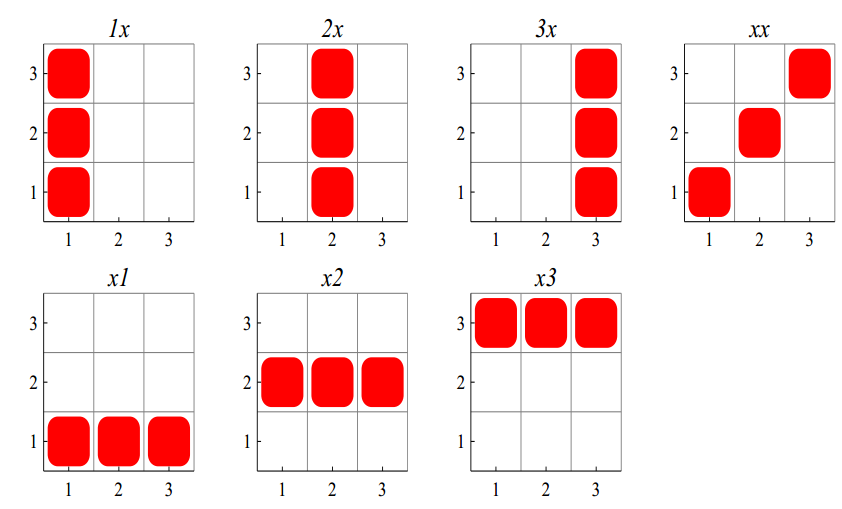
\includegraphics[scale=0.3]{cblines.png}
\caption{Combinatorial lines in $[3]^2$ (Source: \cite{polymath2010density})} \label{cl}
\end{figure}

For $k=3$ and $n=8$, a combinatorial line over alphabets $\{1,2,3\}$ for the word  $w(x)=1xx2x23x$ is the set :
$\{w(x;i)=1ii2i23i: \ i\in [3]\}=  \{11121231, 12222232, 13323233 \}.$ As matrix representation, this combinatorial line can be expressed as:
\begin{center}
$\left(\begin{array}{cccccccc}
1 & 1 & 1 & 2 & 1 & 2& 3 &1\\  1 & 2 & 2 & 2 & 2 & 2 & 3 & 2\\ 1 & 3 & 3 & 2 & 3 & 2 & 3 & 3 
\end{array}  \right)$
\end{center}

%\Jnote{This is not consistent with your previous notation.}

Sets which do not contain any combinatorial line are called  \textit{line-free}.  So, according to \cite{polymath2012new}, the Hales-Jewett is stated as:

\begin{thm}[Hales-Jewett theorem]   For every pair of positive integers $k$ and $r$ there exists a positive number $HJ(k, r)$ such that for every $n \geq HJ(k, r)$ and every $r$-colouring of the set $[k]^n$ there is a
monochromatic combinatorial line.   \label{hj1} 	\end{thm}

There are several proofs of the Hales-Jewett theorem. The original proof has been given by \cite{hales1987regularity}. \cite{shelah1988primitive} proved a primitive recursive\footnote{Primitive recursion is a procedure that defines the value of a function at an argument $n$ by using its value at the previous argument $n-1$.  In a computer, a primitive recursive bound can be implemented only using do-loops (see https://plato.stanford.edu/entries/recursive-functions/$\#1.3$).} bound for the Hales-Jewett number using simple induction.
\cite{nilli1990shelah} presented a compact form of Shelah’s Proof of the Hales-Jewett Theorem.  This condensed form states that for every $k,r \geq 1$, $HJ(k,r) \leq \frac{1}{kr} h_4 (k+m+2)$ with $h_i$  a function defined as: $h_1(n)=2n$; for $i>1$, $h_i=h_{i-1}(h_{i-1}(\ldots h_{i-1}(1))) $ where $h_{i-1}$  is taken  $n$ times.
%\Jnote{s/$h_i$/$h_i(n)$. Also put this formula as separate equation.}

 \cite{matet2007shelah} gave a variant of Shelah’s proof of the Hales–Jewett theorem by replacing Shelah’s pigeonhole lemma by an appeal to the Ramsey’s theorem.

The Hales-Jewett theorem has also a density version. By considering a nonempty subset  $A$ of the set $[k]^n$, the density of $A$ inside $[k]^n$ is a positive real number $\delta=\frac{|A|}{k^n}$. Values of $\delta$ are bounded by $0$ and $1$, specifically  $0< \delta \leq 1.$ 

Let denote by $DHJ(k, \delta)$ the density Hales-Jewett number. The density version of the Hales-Jewett theorem is announced according to \cite{polymath2012new} as follows:

\begin{thm}[Density version of Hales-Jewett theorem]   For any $k \in \mathbb{Z}^+$ and any real number $0< \delta \leq 1$,  there exists a positive integer $DHJ(k, \delta)$ such that if $n \geq DHJ(k,\delta)$ and $A$ is any subset of $[k] ^n$ with $|A| \geq \delta k^n$, then $A$ contains a combinatorial line.  \label{hj2}	\end{thm}

The proof of the density version of the Hales-Jewett theorem has been demonstrated by \cite{furstenberg1991density} using ergodic methods.  \cite{polymath2012new} gave an elementary non-ergodic proof of the density version of the Hales-Jewett theorem by giving a quantitative bound on how large $n$ needs to be and qualified this theorem as one of the fundamental results of Ramsey theory. A simplified version of \cite{polymath2012new} has been given by \cite{dodos2013simple} using  a purely combinatorial proof of the density Hales–Jewett Theorem.

Furthermore, there are four important theorems we have talked about: the Van der Waerden's theorem \eqref{vd1}, the Szemerédi's theorem \eqref{sz1}, the  Hales-Jewett theorem \eqref{hj1} and the density Hales-Jewett theorem \eqref{hj2}. 
In \eqref{vsz} we have shown that the Szemeredi's theorem implies the Van der Waerden's theorem. It is reasonable to show these three implications: the density version of the Hales-Jewett theorem implies the Hales-Jewett theorem, the Hales-Jewett theorem implies the  Van der Waerden's theorem, and the density version of the Hales-Jewett theorem implies the Szemerédi's theorem.

\subsection{Density version of the Hales-Jewett theorem implies the Hales-Jewett theorem}

To show that this density version of Hales-Jewett theorem implies the Hales-Jewett theorem, we need only to set as in  \eqref{vsz}, $\delta=\frac{1}{r}.$ By $r$-colouring the set $[k]^n$, that is by partitioning to $r$ classes,  if $A_{max}$ is the set containing the maximum number then $|A_{max}| \geq \frac{k^n}{r}=\delta k^n.$ Hence, according to \eqref{hj2}, $A_{max}$ contains a combinatorial line.

\subsection{Hales-Jewett theorem implies Van der Waerden's theorem}

To show that the Hales-Jewett theorem implies the Van der Waerden's theorem, we need only to show that combinatorial line corresponds to the arithmetic progression.
%\Jnote{``combinatorial lines correspond to arithmetic progressions''.}
%\Jnote{I'm not sure what you are trying to say here.}

Let us  assume that the Hales-Jewett theorem is true and show that the combinatorial line of $k$ elements contained to the subset $A$ corresponds to the arithmetic progression of length $k$.

We have defined $[k]$ as the set $\{1,2,\ldots, k\}.$ Instead to start by $1$, let us start by $0.$ In this part, $[k]$ expresses the set $\{0,1,\ldots, k-1\}.$ It is obvious that $[k]=\mathbb{Z}/k\mathbb{Z}.$

Let $n$ be the positive number of the Hales-Jewett theorem, that is $n\geq HJ(k,r)$, then the set $[k]^n=(\mathbb{Z}/k\mathbb{Z})^n=\{(y_0,y_1, \ldots, y_{n-1}): \ y_i \in [k] \}$ has $k^n$ elements. Similarly, the set $[k^n]=\{0,1,\ldots, k^n-1\}$ has also $k^n$ elements. Note that the set $[k^n]$ contains natural number.
While, elements of the set $[k]^n$ can be interpreted as 
the digits  in base$-k$ number system of the numbers $\{0,1,\ldots,k^n-1\}.$

Let us consider the bijection $f:[k]^n \longrightarrow [k^n]$ defines as follows:

$$f(y_0,y_1,\ldots, y_{n-1})=y_0+y_1k+y_2 k^2+\ldots+y_{n-1}k^{n-1}.$$

Let $w(x) \in ([k] \cup \{x\})^n\setminus [k]^n$ be an $x$-string. The combinatorial line generates by $w(x)$ is a set of $k$ elements defined by  $\{w(x;i):i\in [k]\}.$  

Let $w(x;i)$ and $w(x;i+1)$ be two consecutive elements of the combinatorial line generates by $w(x)$. We denote  $w(x;i)=(y_{0,i},y_{1,i},\ldots, y_{n-1,i}) $ and $w(x;i+1)=(y_{0,i+1},y_{1,i+1},\ldots, y_{n-1,i+1})$ where  the elements  $y_{j,i} \in [k]$ for $0 \leq j \leq n-1$ and $0 \leq i \leq k-1.$

So, it is obvious that $w(x;i)$ is a vector. By definition of addition in a vector space, the difference between two consecutive elements $w(x;i)$ and $w(x;i+1)$ of this combinatorial line is a constant (vector). Let us call this constant $l=(l_0, l_1, \ldots, l_{n-1})= w(x;i+1)-w(x;i)$.


For $j\in \{0,1,\ldots, n-1\}$, $l_j$ has two values: 
$l_j= \left\lbrace \begin{array}{ll}1 & \text{ if } y_{j,i}\neq y_{j,i+1} \\ 0 & \text{ if } y_{j,i} =  y_{j,i+1}   \end{array} \right. .$
%\Jnote{$l_j=1$ or $l_j=x$?}

Let $w(x;0)=(y_{0,0},y_{1,0},\ldots, y_{n-1,0})$ be the first element of the combinatorial line generated by $w(x)$ . Then, for $0\leq i \leq k-1$ an element $w(x;i)$ of the combinatorial line can be expressed as: $$w(x;i)=w(x;0)+il.$$
%\Jnote{Change o to $0$.}

Let us call  $a$ the image of $w(x;0)$ by $f$, that is $a=f(w(x;0))$ and  $d$ the image of $l$ by $f$, that is $d=f(l).$ $a$ and $d$ are both integers.  We denote by $J$ the set $\{j: \ y_{j,i}\neq y_{j,i+1} \}.$ The integer $d$ can be expressed as:
$$d=f(l)=l_0+l_1k+\ldots+l_{n-1}k^{n-1}=\sum_{j=0}^{n-1}l_jk^j= \sum_{j\in J} k^j.$$
Thus, $f(w(x;i))=a+id$, $a$ and $d$ fixed, $0\leq i \leq k-1$. Hence, the set $\{a+id: \ i\in [k]\}$ forms an arithmetic progression of length $k.$ So, for any combinatorial line of $k$ elements corresponds an arithmetic progression of length $k.$ 
Therefore, the Hales-Jewett theorem implies the Van der Waerden's theorem where $k$ and $r$ are the same .

\subsection{Density version of the Hales-Jewett theorem implies the  Szemerédi's theorem}

We have shown that any combinatorial line of $k$ elements corresponds an arithmetic progression of length $k.$ Also, we have established that there exists a bijection between $[k]^n \longrightarrow [k^n].$ So, we just need to set $N(k,\delta)=k^n$ to show that the Hales-Jewett theorem implies the Szemerédi's theorem where $n\geq DHJ(k,\delta).$
%\Jnote{Stil not fixed. What is $n$ here?}

As we have shown in \eqref{vsz} that the Szemerédi's theorem implies the  Van der Waerden's theorem, we can establish by transitivity that the density version of the Hales-Jewett implies the Van der Waerden's theorem.

\subsection{Density Hales-Jewett number} \label{dhjn}

Let $n \geq 0$ and $k \geq 1.$ The \textit{density Hales-Jewett number}	denoted by $d_{k,n}$ is defined as the size of the largest subset of the set $[k]^n=\{1,2, \ldots, k\}^n$ which contains no combinatorial	line.  Let $W$ be this largest subset, then $d_{k,n}=|W|.$  Note that $W$ is also called a \textit{line-free}. Furthermore, the density of $W$ can also be defined by the quotient $\frac{|W|}{k^n}$. In this case, the density is denoted by $\Delta_{k,n}$, that is  $\Delta_{k,n}=\frac{|W|}{k^n}.$ 

The combinatorial line is to $d_{k,n}$ what the arithmetic progression is to $\delta_{k,N}$ (for the Szemerédi's theorem). That is, the major  difference between $d_{k,n}$ and $\delta_{k,N}$ is located on the definition of the largest subset: combinatorial line for the first and arithmetic progression for the second. 

\cite*{furstenberg1991density} showed that $d_{k,n}=o(k^n)$ (respectively $r_{k,N}=o(k^n)$) as $n\longrightarrow \infty.$
%\Jnote{Rephrase: Density Hales-Jewett theorem is equivalent to saying
It means that $d_{k,n}$ (respectively $r_{k,N}$) grows slower than  any constant fraction of $k^n$.
%\Jnote{Rephrase: ...it means that $d_{k,n}$ grows slower than any constant fraction of $k^n$}.
In another words, the growth rate of $d_{k,n}$ (respectively $r_{k,N}$) is strictly less
%\Jnote{s/less/strictly less}
than the growth rate of $k^n.$

For $k=1$ and $k=2$, the density Hales-Jewett numbers $d_{1,n}$ and $d_{2,n}$ are easier   than other cases.
%\Jnote{Don't say it is trivial for $k=2$. You are not allowed to say it is   trivial if you cannot prove it (can you?). You can say that it is easier   than other cases.}
Thus, $d_{1,n}=1$ and $d_{2,n}= {n \choose \lfloor \frac{n}{2} \rfloor}$ where $\lfloor x \rfloor $ is the floor function. 
% defined as following: $\lfloor x \rfloor =n \Longleftrightarrow n \leq x < n+1 \Longleftrightarrow  x-1 < n \leq x .$
%\Jnote{Definition of floor is not correct (you have to say $n$ is integer).  You can delete it anyway.}

\cite{polymath2010density} used both human and computer-assisted arguments to compute some non-trivial density Hales-Jewett numbers for $k=3$ when $n= 0,\ldots,6.$

\begin{table}[h]
\centering
\begin{tabular}{|c|c|c|c|c|c|c|c|}
\hline 
$\mathbf{n}$ & 0 & 1 & 2 & 3 & 4 & 5 & 6 \\ 
\hline 
$\mathbf{d_{3,n}}$ & 1 & 2 & 6 & 18 & 52 & 150 & 450 \\ 
\hline 
\end{tabular}
\caption{Some known values of $d_{3,n}$ for $ n= 0,\ldots,6.$}
\end{table} 

Let us give examples of the line-free derived from \cite{polymath2010density} for $k=3$ and $n=2$ and $n=3.$
\begin{itemize}
\item For $n=2$, there are 4 largest line-free of $[3]^2$ each with cardinality $d_{3,2}=6 :$ 

$ \{12, 13, 21, 22, 31, 33 \}$, $\{11, 12, 21, 23, 32, 33 \}, \{11, 13, 22, 23, 31, 32 \}, \{12, 13, 21, 23, 31, 32 \}.$
\item For $n=3$, the largest line-free of $[3]^3$ with cardinality $d_{3,3}=18$ is: 

$\{112, 113, 121, 122, 131, 133, 211, 212, 221, 223, 232, 233, 311, 313, 322, 323, 331, 332 \}.$
\end{itemize}
%\Jnote{Fix too long lines here.}

Knowing that $d_{3,0}=1$, $d_{3,1}=2$,  \cite{polymath2010density} gave an upper bound of $d_{3,n}$ for $n= 0,\ldots,6$: $$d_{3,n+1} \leq 3 d_{3,n}$$

and for large $n$ and for $k\geq 3$, $d_{k,n} \geq k^n \exp \left(-O(\log n)^{1/l}\right)$ where $\ell$ is the largest integer such that $2k > 2^{\ell}$. This lower bound can simply be written as: $d_{k,n} \geq k^n  \exp \left(-O(\log n)^{1/\lceil \log_2 k \rceil}\right)$ where $\lceil x \rceil$=ceilling$(x)$ is the least integer greater than or equal to $x.$ 

This density Hales-Jewett number will be helpful to establish the connection between parallel repetition and the Hales-Jewett theorem.The next chapter deals with the parallel repetition of multi-prover games.
%
%For $k=2$, the density Hales-Jewett number is: $\Delta_{2,n}=\Theta(1/\sqrt{n})$ known by Sperner's theorem.

%\cite{polymath2010density} presented some approximations of the lower and upper bounds for general case of $d_{k,n}.$
%
%The proof of the theorem has been given by \cite{furstenberg1991density} without explicit bounds. \cite{polymath2012new} gave an upper bound of $\Delta_{k,n}$ for a particular case ($k=3$): $\Delta_{3,n} \leq O(1/\sqrt{\log^* n}).$ Previously, a lower  density Hales-Jewett bound  was known through the work of \cite{polymath2010density} who establishes that  
% 
 
 
















%The idea is to let  $ N_0=\ell^{n_0}$, and to associate with every number in $ [N]$ the digits in its expansion in the base-$ \ell$ number system. Then any combinatorial line would correspond to an arithmetic progression. (But not conversely. Why?)




